\chapter{Используемые технологии}
\section{Структура проекта ВСТАВИТЬ ИМЯ ТАБЛИЦЫ В КОНЦЕ БЕСИТ КОМПЛИЯЦИЯ}
Так как исходных кодов библиотек нет, значит возможности перевести их на ActionScript нет. Было принято решение использовать виртуальный сервер для связи Flash с динамическими библиотеками. На рис. ~\ref{scheme1} представлена схема работы нашего проекта.\\
\begin{figure}[!ht]
	\begin{center}
		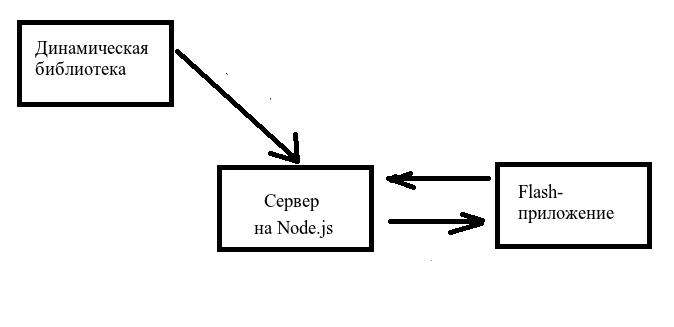
\includegraphics[width=12cm]{schemeOfCommunic}
	\end{center}
	\caption{Схема связи Динамической библиотеки и Flash-приложения}
	\label{scheme1}
\end{figure}

Этапы запуска приложения:
 \begin{itemize}
        \item Запуск сервера,
        \item Иницилизация динамической библиотеки,
        \item Запуск Flash-приложения;
    \end{itemize}

После этого Flash-приложение посылает запрос серверу на выполнение той или иной, загруженной из динамической библиотеки, функции. Сервер обрабатывает запрос, выполняет нужную функцию с полученными из запроса параметрами, и посылает ответ клиенту (Flash-приложению). 
Данная схема позволяет Flash-приложениям использовать динамические библиотеки.

\section{Выбор платформы для Flash}
В качестве среды программирования мною был использована среда IntelliJ IDEA (рис. ~\ref{inteliJ}).
\begin{figure}[!ht]
	\begin{center}
		
\includegraphics[width = 8cm]{intelliJ}
	\end{center}
	\caption{Эмблема IntelliJ IDEA}
	\label{inteliJ}
\end{figure}
Она была выбрана, так как она является удобной платформой для создания приложений, в ней существует большой набор мощных инструментов, не навязывающих определенных структур проекта, имеет удобный редактор. В качестве компилятора был выбран Flex SDK. По сравнению с компилятором Adobe Flash, он имеет удобный debugger, сохраняя при этом все возможности Flash. В отличие от Adobe Flash Flex SDK распространяется бесплатно.

\section{Выбор платформы для создания сервера}
\subsection{Протокол передачи} 
В качестве протокола передачи информации был выбран http-протокол, потому что он, как правило, не должен перекрываться для передачи информации. Это происходит, потому что для открытия веб-страницы в интернете требуется этот протокол, следовательно ни в какой операционной системе он не запрещён к использованию.
Также в ActionScript существует класс URLLoader, который относится к пакету flash.net. Данный класс может создавать http-запросы и принимать их в виде текста, двоичных данных или переменных в кодировке URL. Этот класс полностью удовлетворяет потребностям проекта.

\subsection{Среда создания}
Сервер может располагаться локально на компьютере участника, либо находиться удаленно.
Было принято решение размещать сервер локально на каждом компьютере, на котором будет устанавливаться пакет конкурса КИО. Плюсы данного варианта заключаются в том, что участникам не нужно постоянное устойчивое соединение с удалённым сервером для посылки запросов. Тем самым, ученики могут скачать установщик и учавствовать в конкурсе, пользуясь компьютерами без выхода в интернет. Минус — нужно найти такой сервер, который не будет занимать много места, будет быстро скачиваться, и будет легок в настройке, быстр в использовании.
Существует большое количество платформ и языков программирования для создания серверов, а именно: 
C++, PHP, node.js, python. 
Рассмотрим примеры создания серверов на этих платформах. 
\paragraph{Сервер на С++}
В листинге ~\ref{httpC} реализован простой http-сервер, который на успешный запрос клиента отвечает, что сообщение было получено. Программисту, который никогда не сталкивался с созданием серверов будет достаточно сложно разобраться в назначении многих параметров и вообще структуры создания сервера на C++.

В тоже время сервер на C++ является хорошим вариантом для нашего проекта, так как он не будет занимать много места на жёстком диске и будет достаточно быстр при обработке для наших условий.
 \lstinputlisting[frame=shadowbox,
   emph={forsuffixes,text,bpath},emphstyle={\color{red}},
   emph={[2]fill,unfill},emphstyle={[2]\bfseries\underbar}, caption=Пример http-сервера на С++, label={httpC}
 ]{httpC.c}

\paragraph{Сервер на PHP}
Теперь рассмотрим пример http-сервера на PHP. Последняя версия PHP 5.4 содержит встроенный веб-сервер, соответственно не требуется установка Apache или других аналогичных серверов, которые сложны в настройке.
Запускается сервер следующим образом. Пример для Linux:
 \begin{lstlisting}[numbers=none, language=bash]
	$ php -S localhost:8000
\end{lstlisting}
В консоли выведется следующее:
 \begin{lstlisting}[numbers=none, language=bash]
	PHP 5.4.0 Development Server started at Date
	Listening on localhost:8000
	Document root is /home/username/
	Press Ctrl-C to quit
\end{lstlisting}
Скрипт index.php будет выглядеть так:
 \begin{lstlisting}[numbers=none, language=PHP]
<?
  echo "Hello world!";
\end{lstlisting}
На каждый запрос, посланный серверу, будет выдаваться содержимое index.php, в данном примере будет выводиться Hello world!

\paragraph{Сервер на Python}
В коде листинга ~\ref{httpPython} сервер обрабатывает запрос, и при успешном запросе выдаёт клиенту запрошенную страницу.
 \lstinputlisting[frame=shadowbox, language=Python,
   emph={forsuffixes,text,bpath},emphstyle={\color{red}},
   emph={[2]fill,unfill},emphstyle={[2]\bfseries\underbar}, caption=Пример http-сервера на Python, label={httpPython}
 ]{httpPython.py}

Сервер на Python умеет отвечать на запрос с именем страницы выводом самой страницы.

\paragraph{Сервер на Node.js}
Node.js — это сравнительно новая платформа, построенная на основе  Chrome's JavaScript Runtime для легкого создания быстрых, масштабируемых сетевых приложений. Node.js позволяет выполнять Javascript-код вне браузера. Он состоит из среды исполнения программ и большого количество дополнительных библиотек. Листинг ~\ref{httpNodejs} отражает код для создания сервера на Node.js
 \lstinputlisting[frame=shadowbox, language=Java,
   emph={forsuffixes,text,bpath},emphstyle={\color{red}},
   emph={[2]fill,unfill},emphstyle={[2]\bfseries\underbar}, caption=Пример http-сервера на Node.js, label={httpNodejs}
 ]{httpNode.js}

Все. Вот и весь сервер. На каждый запрос он выводит Hello World. Очень просто и понятно. К неоспорим плюсам относится то, что процесс node.js живёт долго и обрабатывает все http-запросы внутри себя. Это значит, что для каждого нового запроса не выполняется инициализация, как, например, на PHP. А это существенно сокращает время обработки запросов. С помощью таких инструментов как The Node Toolbox (http://toolbox.no.de/) и npm (http://npmjs.org/) процесс поиска, выбора и установки необходимых модулей становится простым и быстрым. Также очень понравилась документация, которая существует не только на английском, но и на русском языках.
Заглядывая в будущее, если предположить, что сервер будет запускаться удалённо, тогда не нужна никакая настройка сервера локально на каждом компьютере. Но тогда будет возникать проблема перегруженности сервера, ведь в предыдущие года в конкурсах участвовали более 60 тысяч учеников и их число каждый год растёт. \\
Node.js выполняет все запросы асинхронно. Если какой-то запрос приходит на сервер, а сервер уже занят обработкой другого процесса, то новый запрос всё равно сразу же начнёт выполняться. Быстродействие node.js впечатляет.\\
Приведу сравнительный анализ, представленный на сайте \\
http://b.brainscode.com/2011/04/nodejs-vs-php.html. В этом анализе сравнивается быстродействия node.js и php. Проведем тесты на простых математических вычислениях. В листингах ~\ref{phpTest} и ~\ref{nodejsTest} предсталены скрипты тестов на PHP и Node.js соответственно.
 \lstinputlisting[frame=shadowbox, language=PHP,
   emph={forsuffixes,text,bpath},emphstyle={\color{red}},
   emph={[2]fill,unfill},emphstyle={[2]\bfseries\underbar}, caption=Тестовый скрип php, label={phpTest}
 ]{phpTest.py}
 \lstinputlisting[frame=shadowbox, language=Java,
   emph={forsuffixes,text,bpath},emphstyle={\color{red}},
   emph={[2]fill,unfill},emphstyle={[2]\bfseries\underbar}, caption=Тестовый скрип Node.js, label={nodejsTest}
 ]{nodejsTest.js}

Таблица ~\ref{testTable} показывает результаты тестов.

\begin{center}
\begin{tabular}{|c|c|c|}
\hline
  & \multicolumn{2}{|c|}{\textbf{Время (сек.)}}\\
\hline
\textbf{Кол-во итераций} &   \textbf{Php}     &  \textbf{Node.js}\\
\hline
100 000 & 0.077 & 0.02\\
\hline
1 000 000 & 0.759 & 0.016\\
\hline
10 000 000 & 7.605 & 0.157\\
\hline
100 000 000 & 75.159 & 1.567\\
\hline
\end{tabular}
\end{center}
%\tablecaption{Таблица ~\ref{testTable}. Сравнение быстродействия PHP и Node.js} \label{testTable}

Как видим nodejs существенно превосходит в данном тесте, при самой большой размерности выигрыш в времени выходит почти в 50 раз, при значении в 100 000 раз этот показатель равен — 38 соответственно. Выигрыш, как видно существенный.
Также в видео-лекции Ryan'а Dahl'а (одного из создателей Node.js) показано, что если создан сервер, который на каждый запрос отвечает двух-секундной задержкой (см. ~\ref{dahl}), то при 100 000 одновременных запросах время обработки запросов сервером будет составлять чуть более 2 секунд, что свидетельствует о параллельной обработке запросов, об асинхронной работе сервера. 
\begin{lstlisting}[numbers=none, language=bash, caption =Тело функции обработки запроса в Node.js]
  setTimeout(function(){
	console.log("hello world");
}, 2000);
\end{lstlisting}

И, в конце-концов, программы на Javascript являются легко читаемыми.

По вышеперечисленным причинам было принято решение использовать сервер, созданный на node.js. Из минусов можно отметить, что сервер будет занимать чуть менее 5 мб, но, учитывая все достоинства использования Nodejs, этим минусом можно пренебречь. Даже если предположить, что у участника интернет типа dial-up с максимальной скоростью 64 кбит/сек:
\begin{itemize}
 \item 64 кбит/сек = 8 кбайт/сек;
  \item 5 мбайт = 5120 кбайт  (максимальный размер сервера)
  \item 5120 / 8 = 640 сек;
  \item 640 / 60 = 10 минут 40 секунд - худший расклад.
\end{itemize}
При скорости 512 кбит/сек (64 кбайт/сек) время закачки будет равно 80 секундам.
\subsection{Создание тестовой динамической библиотеки}\label{CreationDynLib}
Также для создания тестовой динамической библиотеки будет использоваться Microsoft Visual Studio 2010 Express для Windows и компилятор gcc на Linux.
В листинге ~\ref{big.c} приведен код, из которого комплируется динамическая библиотека.
 \lstinputlisting[frame=shadowbox, language=Java,
   emph={forsuffixes,text,bpath},emphstyle={\color{red}},
   emph={[2]fill,unfill},emphstyle={[2]\bfseries\underbar}, caption=Код компилируемой динамической библиотеки, label={big.c}
 ]{../f1.c}
Чтобы создать динамическую библиотеку нужно сначала скомпилировать файл big.c. Для этого в терминале вводим следующее:
\begin{lstlisting}[numbers=none, language=bash]
    gcc -fPIC -с big.c
\end{lstlisting}
Ключ -fPIC включен, потому что мы создаём динамическую библиотеку. Это нужно для того, чтобы переходы в функциях использовали не абсолютную адресацию, а относительную, иначе несколько различных программ не смогут использовать эту библиотеку.
В результате мы получаем файл big.o, который используем следующим образом:
\begin{lstlisting}[numbers=none, language=bash]
    gcc -shared -o big.o
\end{lstlisting}
В результате будет получен файл big.so, который и будет являться динамической библиотекой, которая будет использована далее в проекте.
\newpage
\section{Структура проекта}
После того как все языки программирования были выбрана структура проекта будет иметь вид как на рис. ~\ref{schemeWithBranch}. К Node.js подключается дополнительная библиотека node-ffi для работы с динамическими библиотеками. Общение Flash-приложения с сервером происходит через http-запросы и http-ответы. 
Библиотека node-ffi является дополнительной библиотекой Node.js. Принцип ее работы описан в разделе ~\ref{ServerPart}.

\begin{figure}[!ht]
	\begin{center}
		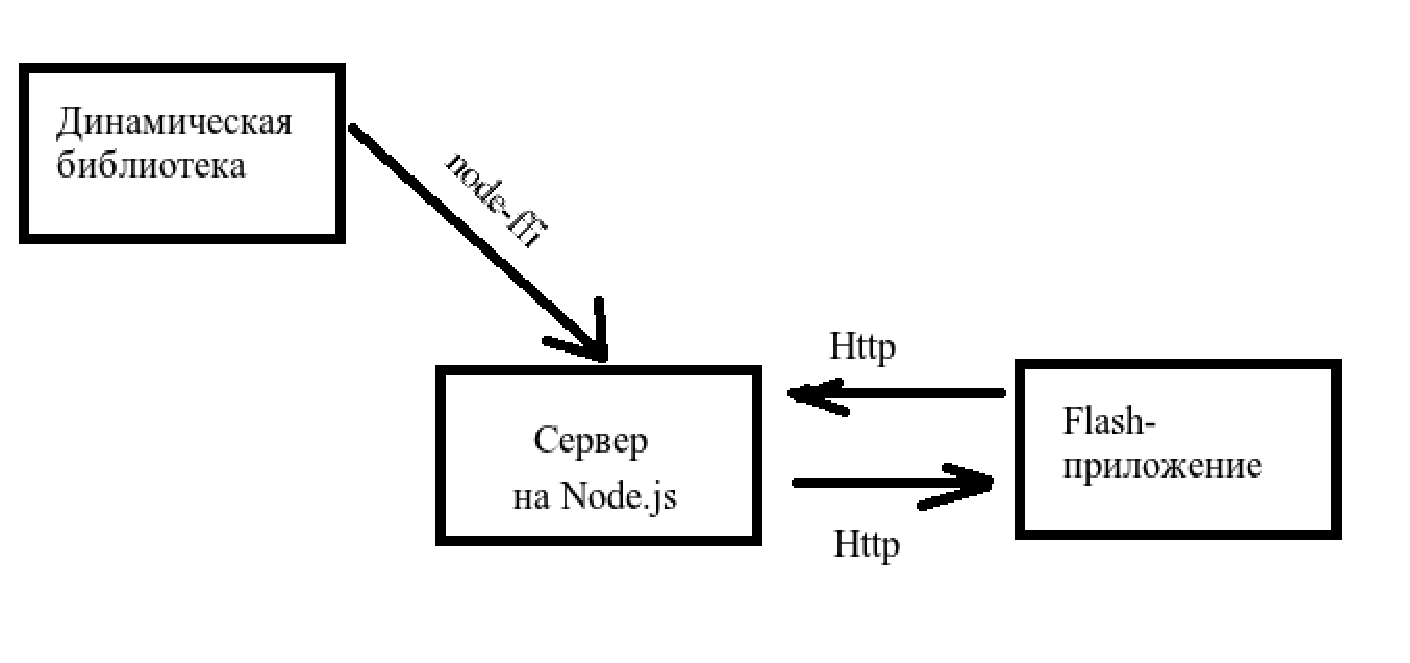
\includegraphics[width=12cm]{schemeOfCommunicWithBranches}
	\end{center}
	\caption{Структура проекта со связями}
	\label{schemeWithBranch}
\end{figure}